\documentclass[12pt, a4paper]{article}
\usepackage{graphicx} % Required for inserting images
\usepackage[final]{pdfpages}
\usepackage[serbian]{babel} % Use the Serbian language package
\usepackage{fontspec} % Required for using system fonts
\usepackage{geometry} % Required for setting page size
\usepackage{fancyhdr} % Required for custom headers and footers
\usepackage[scaled]{helvet}
\usepackage{csquotes}
\usepackage[fixlanguage]{babelbib}
    \bibliographystyle{babunsrt}


% \setmainfont{Nimbus Sans L}
\setmainfont{Roboto}

\setlength{\parindent}{0pt}
\setlength{\parskip}{12pt}%

\geometry{a4paper, margin=1in}

% Customize headers and footers
\pagestyle{fancy}
\fancyhf{} % Clear header and footer
\fancyfoot[R]{\thepage} % Right align page number in the footer
\renewcommand{\headrule}{} % Remove header line


\begin{document}

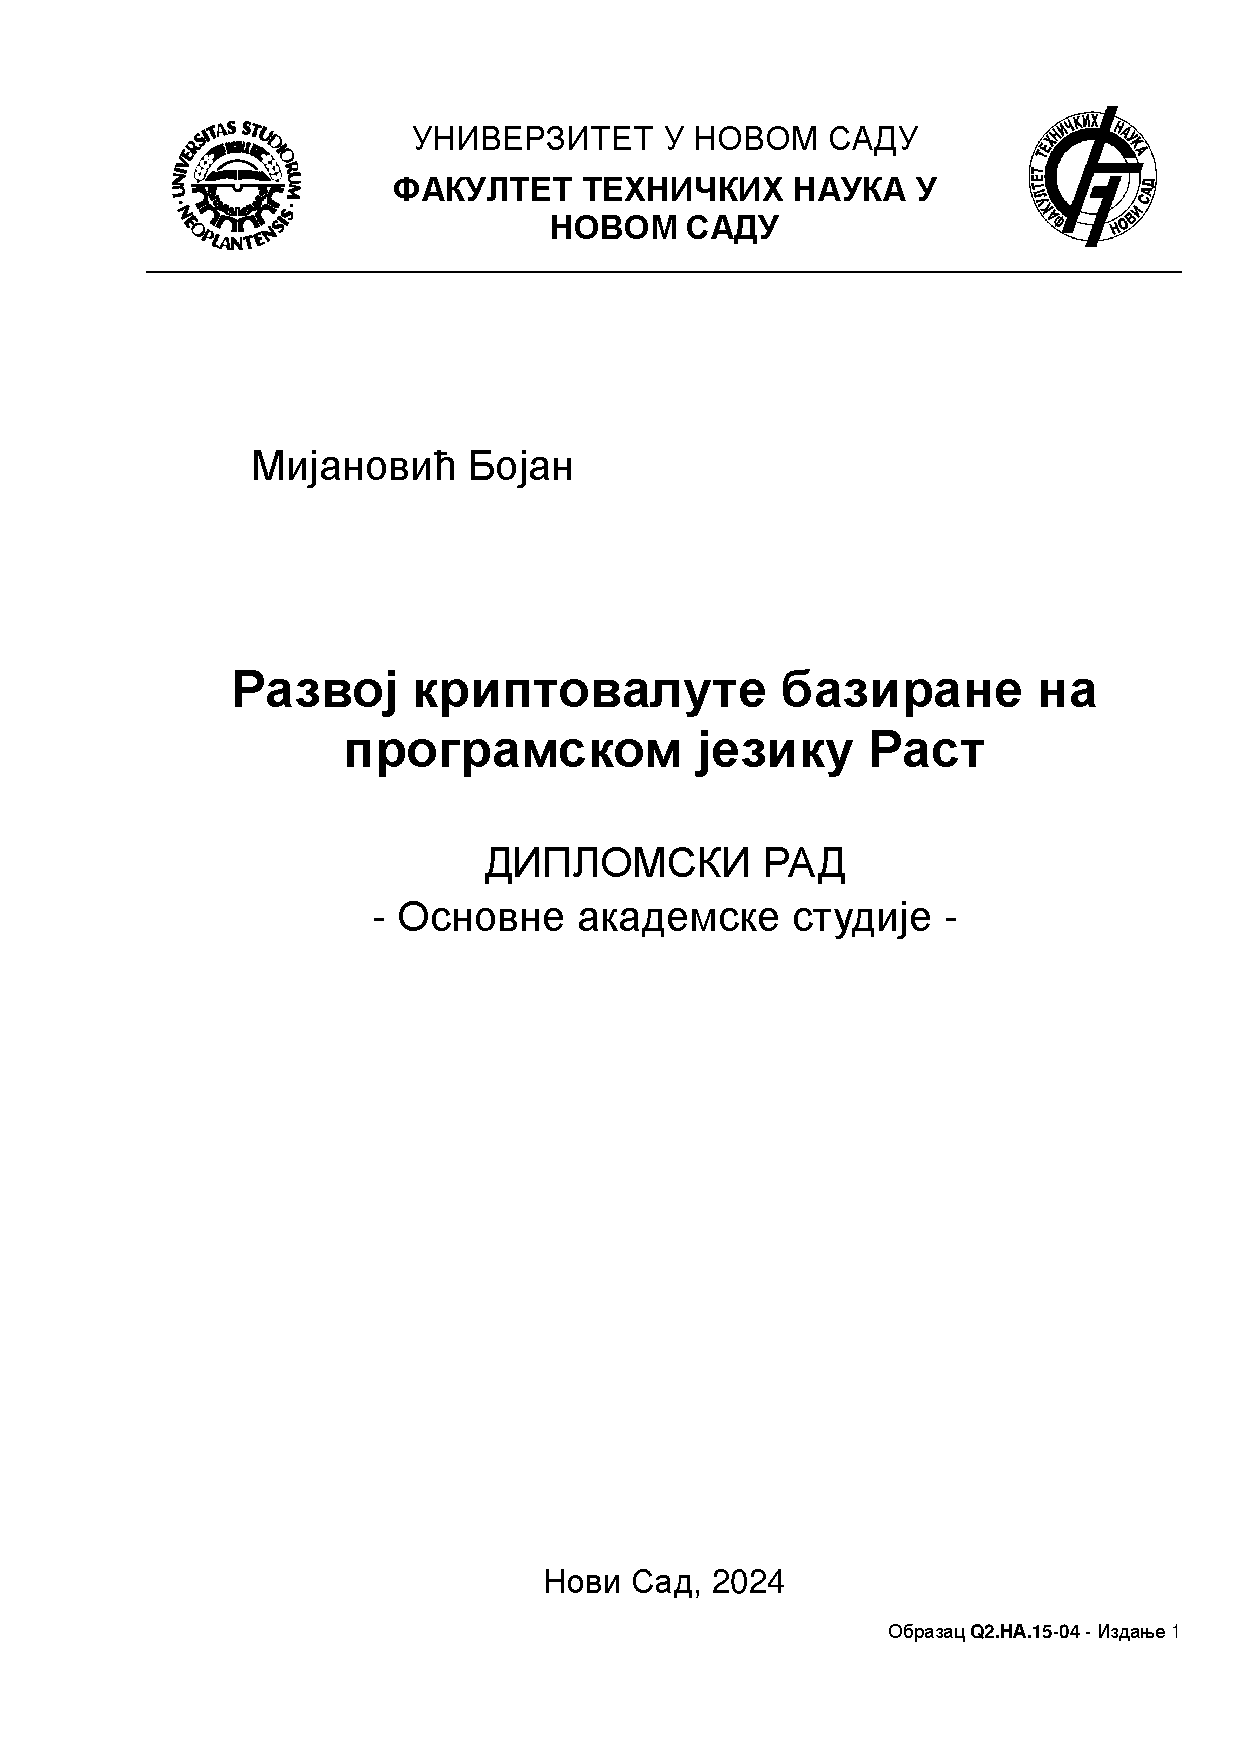
\includepdf[pages=-]{prva_strana.pdf}

\renewcommand{\contentsname}{Садржај}
\tableofcontents
\pagebreak

\section{Увод}
\textit{Blockchain} технологија представља дистрибутивну, децентрализовану и јавну базу свих трансакција \cite{1}.


Први концепт \textit{blockchain} технологије помиње се у 1982. години, када је Давид Чаум у својој дисертацији описао дистрибуирану базу података која користи криптографију \cite{2}. Овај рани рад није био директно повезан са дигиталним валутама, али је поставио темеље за будући развој \textit{blockchain} - а.

Права револуција долази 2008. године када Сатоши Накамото објављује рад "\textit{Bitcoin}: \textit{Peer-to-peer} електронски готовински систем", уводећи први модерни \textit{blockchain} и криптовалуту \textit{Bitcoin}. Генесис блок, први блок \textit{Bitcoin blockchain} - а, ископан је 3. јануара 2009. године, означавајући почетак \textit{blockchain} технологије какву данас познајемо \cite{3}.

\textit{Etherium}, лансиран 2015. године од стране Виталика Бутерина, увео је паметне уговоре који омогућавају сложеније трансакције и аутоматизацију различитих процеса. Овај развој проширио је примену \textit{blockchain} технологије далеко изван дигиталних валута, омогућавајући креирање децентрализованих апликација.

\textit{Blockchain} технологије су се од свог настанка имплементирале у различитим програмским језицима и окружењима. У својим раним фазама, \textit{blockchain} технологије су се углавном развијале користећи језике као што су \textit{C++} и \textit{Java}, захваљујући њиховој ефикасности и широкој употреби у индустрији. Касније, с појавом паметних уговора, \textit{Solidity} је постао стандард за развој на \textit{Etherium} платформи.

Овај рад се фокусира на имплементацију основних концепата \textit{blockchain} технологије у програмском језику \textit{Rust}, који је познат по својој сигурности, перформансама и могућности превенције грешака при руковању меморијом.

Рад је структуиран X целина




\pagebreak

\section{Литература}
\renewcommand{\refname}{}
\vspace{-\parskip} % Remove extra space added by \parskips
\vspace{-\parskip} % Remove extra space added by \parskips
\vspace{-\parskip} % Remove extra space added by \parskips
\vspace{-\parskip} % Remove extra space added by \parskips
\bibliography{bibliography}



\end{document}

